\documentclass[a4paper,12pt]{article}

% Packages
\usepackage{fancyhdr}  % For custom headers and footers
\usepackage{graphicx}  % For including images
% Packages to improve control over figure placement
\usepackage{float}       % [H] placement specifier (exact placement)
\usepackage{placeins}    % \FloatBarrier to prevent floats moving past a barrier
\usepackage{caption}     % Improved caption control
\usepackage{subcaption}  % Sub-figures support
% Optional: absolute positioning on the page
\usepackage[absolute,overlay]{textpos} % precise placement with \begin{textblock*}{width}(x,y)
% Optional: wrap text around figures
\usepackage{wrapfig}
\usepackage{lipsum}    % For placeholder text
\usepackage{amsmath}   % For advanced math typesetting
\usepackage{tabularx}  % For advanced tables

% Logo and Header Configuration
\pagestyle{fancy}
\fancyhf{}  % Clear default header and footer
\fancyhead[R]{
\includegraphics[width=3cm]{img/logo.png}}  % Add your logo here

% Margins
\setlength{\headheight}{52pt}  % Adjust to fit your logo height if needed

% Usage notes:
% - Use \begin{figure}[H] to place a figure exactly where it appears in the source (requires package 'float').
% - Use \FloatBarrier (from 'placeins') to prevent previous floats from moving past that point.
% - For absolute positioning: use the 'textpos' package and \begin{textblock*}{<width>}[<anchor>](<x>,<y>) ... \end{textblock*}.
%   Coordinates are in units set by \TPHorizModule and \TPVertModule (defaults are 1pt); you can set \setlength{\TPHorizModule}{1mm} etc.
% - For wrapping text around an image use \begin{wrapfigure}{r}{0.4\textwidth} ... \end{wrapfigure}.

\title{AudioCLIP4Rec}
\author{Fontana Emanuele}

\begin{document}

\maketitle

\tableofcontents
\newpage

\section{Multimodal Recommender System}
\subsection{Recommender Systems}
With \textbf{Recommender Systems} we refer to all those techniques that have the effect of guiding users in personalized way to interesting objects in a large space of possible options\cite{Lops2011}. There are diffent types of Recommender Systems:
\begin{itemize}
    \item \textbf{Content-Based Filtering}: This approach recommends items similar to those the user has liked in the past. It uses item features and user preferences to make recommendations.
    \item \textbf{Collaborative Filtering}: This method recommends items based on the preferences of similar users. It can be user-based or item-based.
    \begin{itemize}
        \item \textbf{User-Based Collaborative Filtering}: This method finds users with similar preferences and recommends items they have liked.
        \item \textbf{Item-Based Collaborative Filtering}: This method finds items similar to those the user has liked and recommends them. With respect to Content-Based Filtering, this method doesn't use item features to make recommendations.
    \end{itemize}
    \item \textbf{Hybrid Methods}: These methods combine multiple recommendation techniques to improve accuracy and overcome the limitations of individual approaches.
    \item \textbf{Knowledge-Based Recommender Systems}: These systems use explicit knowledge about users and items to make recommendations.
    \item \textbf{Context-Aware Recommender Systems}: These systems take into account contextual information, such as time, location, or social context, to provide more relevant recommendations.
\end{itemize}

\begin{figure}[H]
    \centering
    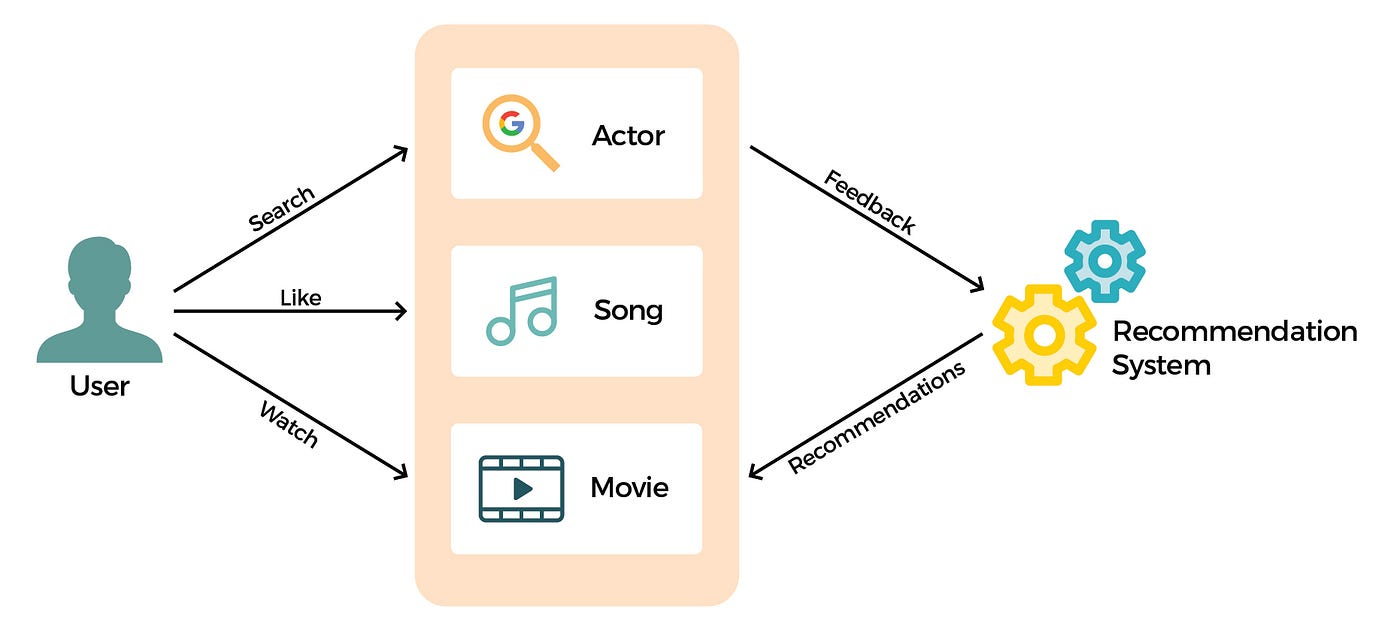
\includegraphics[height=0.2\textheight ,width=0.8\textwidth]{img/RecSys.png}
    \caption{Conceptual representation of a Recommender Systems}
\end{figure}

Recommender Systems are not perfect. They can suffer of several problems like:
\begin{itemize}
    \item \textbf{Cold Start Problem}: Because new users often have very few records in the system, it is hard to guess their preferences given the insufficient information\cite{ColdStart}
    \item \textbf{Data Sparsity}: Most users use the system but do not give rating for feedback to the system in a proper way.\cite{Sparsity}. In addition, in many real-word application we have thousand if not milion of user and item, so it's impossible to think that all user with interact with all item.
    \item \textbf{Scalability}: As the number of users and items increases, the computational complexity of recommendation algorithms can become a challenge. So we can divide scalability problems in two categories: 
    \begin{itemize}
        \item \textbf{Software Scalability}: There's a need to develop algorithms that can handle milions of users and items
        \item \textbf{Hardware Scalability}: There's a need to create systems with powerful hardware that can handle the computational cost in time and space
    \end{itemize}
    \item \textbf{Over Specialization }: Sometimes Recommender algorithms can "overfit" users' preferences, which lead to suggest items that are too similar to those already liked by the user not allowing him/her to discover new items that might be relevant
\end{itemize}


\subsection{Multimodal Recommender Systems}
Differently from classical recommendation approaches, multimodal recommendation exploits multimodal side information about items to enrich the interaction matrix, alleviating its sparsity, and to better understand the content to be recommended; these advantages, in general, lead to more accurate and precise recommendations\cite{Spillong}. We can think about different types of multimodal information: \textbf{Text} in natural language that can be used in every context, \textbf{Audio} for Music, \textbf{Images} for products such as clothes or fornitures, \textbf{Videos} for movies and so on.


The powerfulness of multimodal recommendation is given by the fact that different modalities can provide information about the same item from different perspectives. For example, in a movie recommender system, the textual description of a movie can provide information about its plot, screenshots from the film can provide visual clues about the style of photography and the type of film (animated, live-action, stop-motion, etc.)


Some DNN architectures known as \textbf{Encoders} are used to extract features from different modalities that can be used in different ways like:
\begin{itemize}
    \item \textbf{Concat}: Refers to the concatenation of multimodal features. \cite{ConcatFeature}
    \item \textbf{Fusion and attention}: Refers to the attention mechanisms (like self-attention) to combine multimodal features. \cite{Fusion}
    \item \textbf{GNNs}: They use Graph Neural Networks to model the relationships between items and users, incorporating multimodal features into the graph structure
\end{itemize}

\begin{figure}[H]
    \centering
    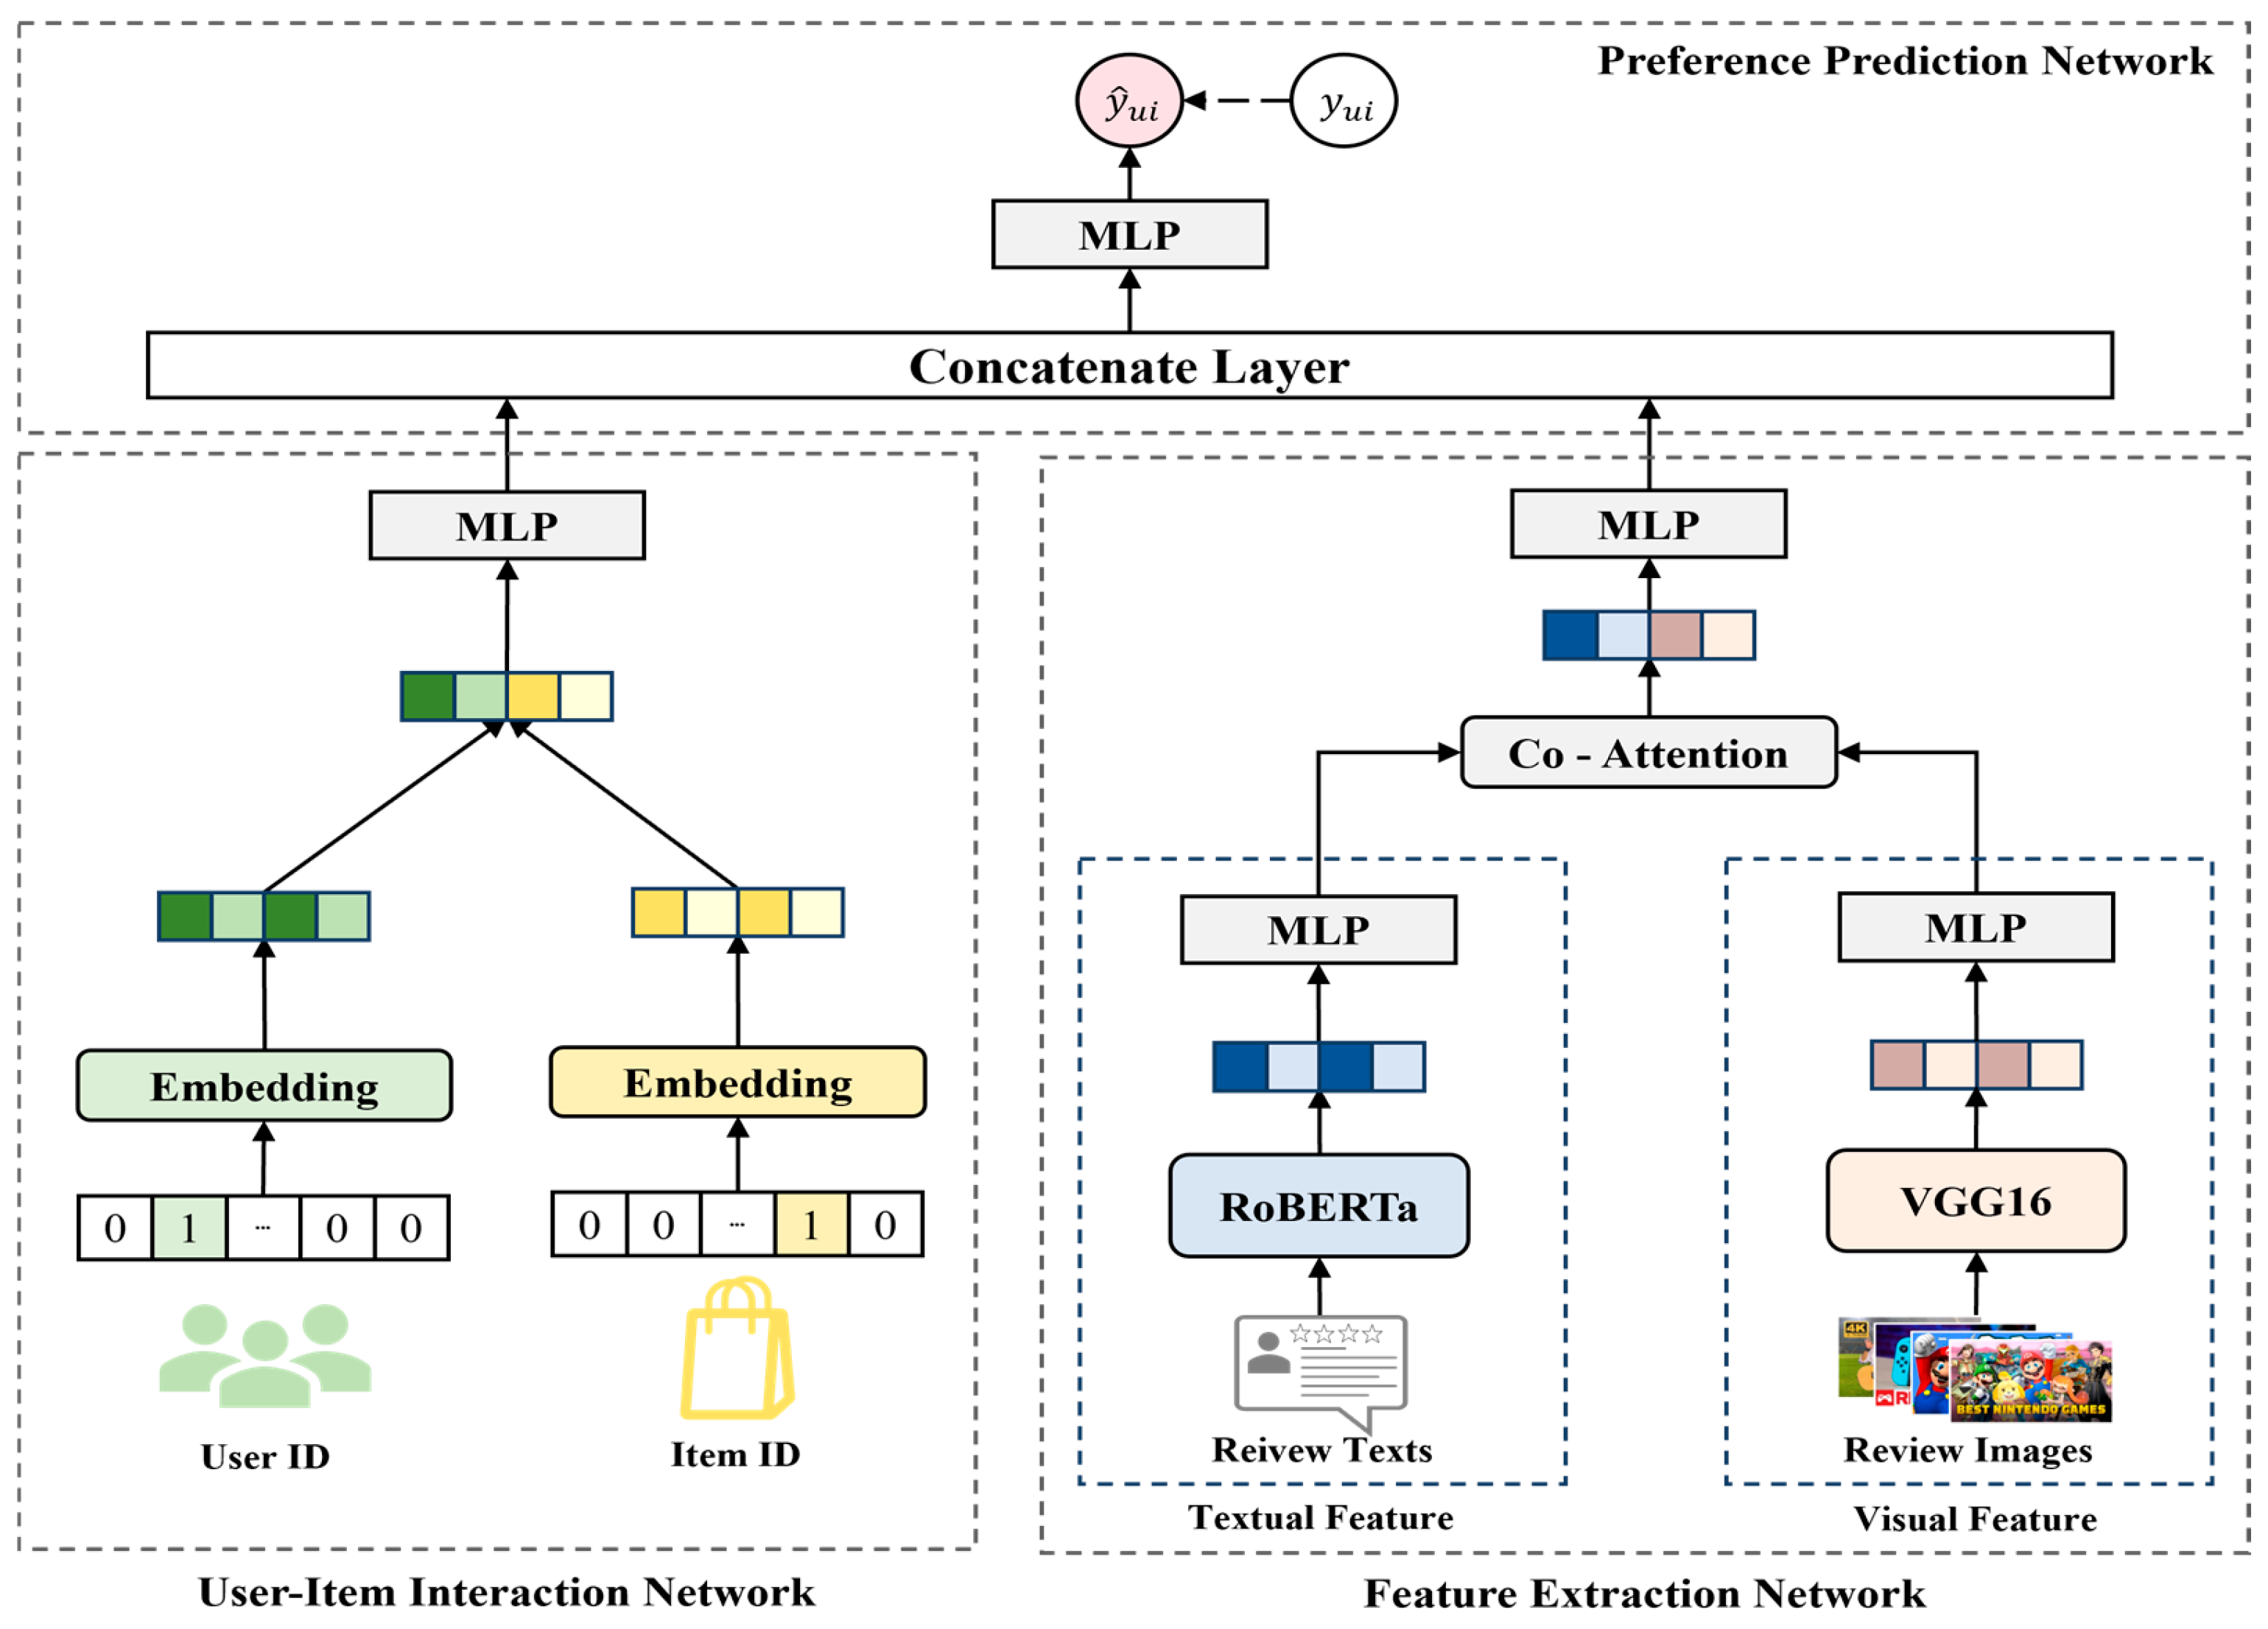
\includegraphics[height=0.5\textheight ,width=0.8\textwidth]{img/MMRec.png}
    \caption{Conceptual representation of a Multimodal Recommender Systems}
\end{figure}
\newpage
\section{Contrastive Learning and AudioCLIP}

\subsection{Contrastive Learning}
Contrastive Learning is self-supervised representation learning by training a model to differentiate between similar and dissimilar samples.\cite{ContrastiveLearning}. In few words, contrastive learning is a technique used to learn a feature space where similar samples are close together and dissimilar samples are far apart. To achieve this, a specific loss function known as \textbf{Contrastive Loss} is used:
\begin{equation}
\ell_{i,j} = -\log \frac{\exp(\text{sim}(z_i, z_j)/\tau)}{\sum_{k=1}^{2N} [k \neq i] \exp(\text{sim}(z_i, z_k)/\tau)},
\end{equation}
where $\text{sim}(z_i, z_j)$ represents the similarity between two feature vectors $z_i$ and $z_j$, $\tau$ is a temperature parameter, and $N$ is the batch size. The numerator focuses on the similarity between the positive pair $(z_i, z_j)$, while the denominator normalizes over all pairs excluding $z_i$ itself.

\begin{figure}[H]
    \centering
    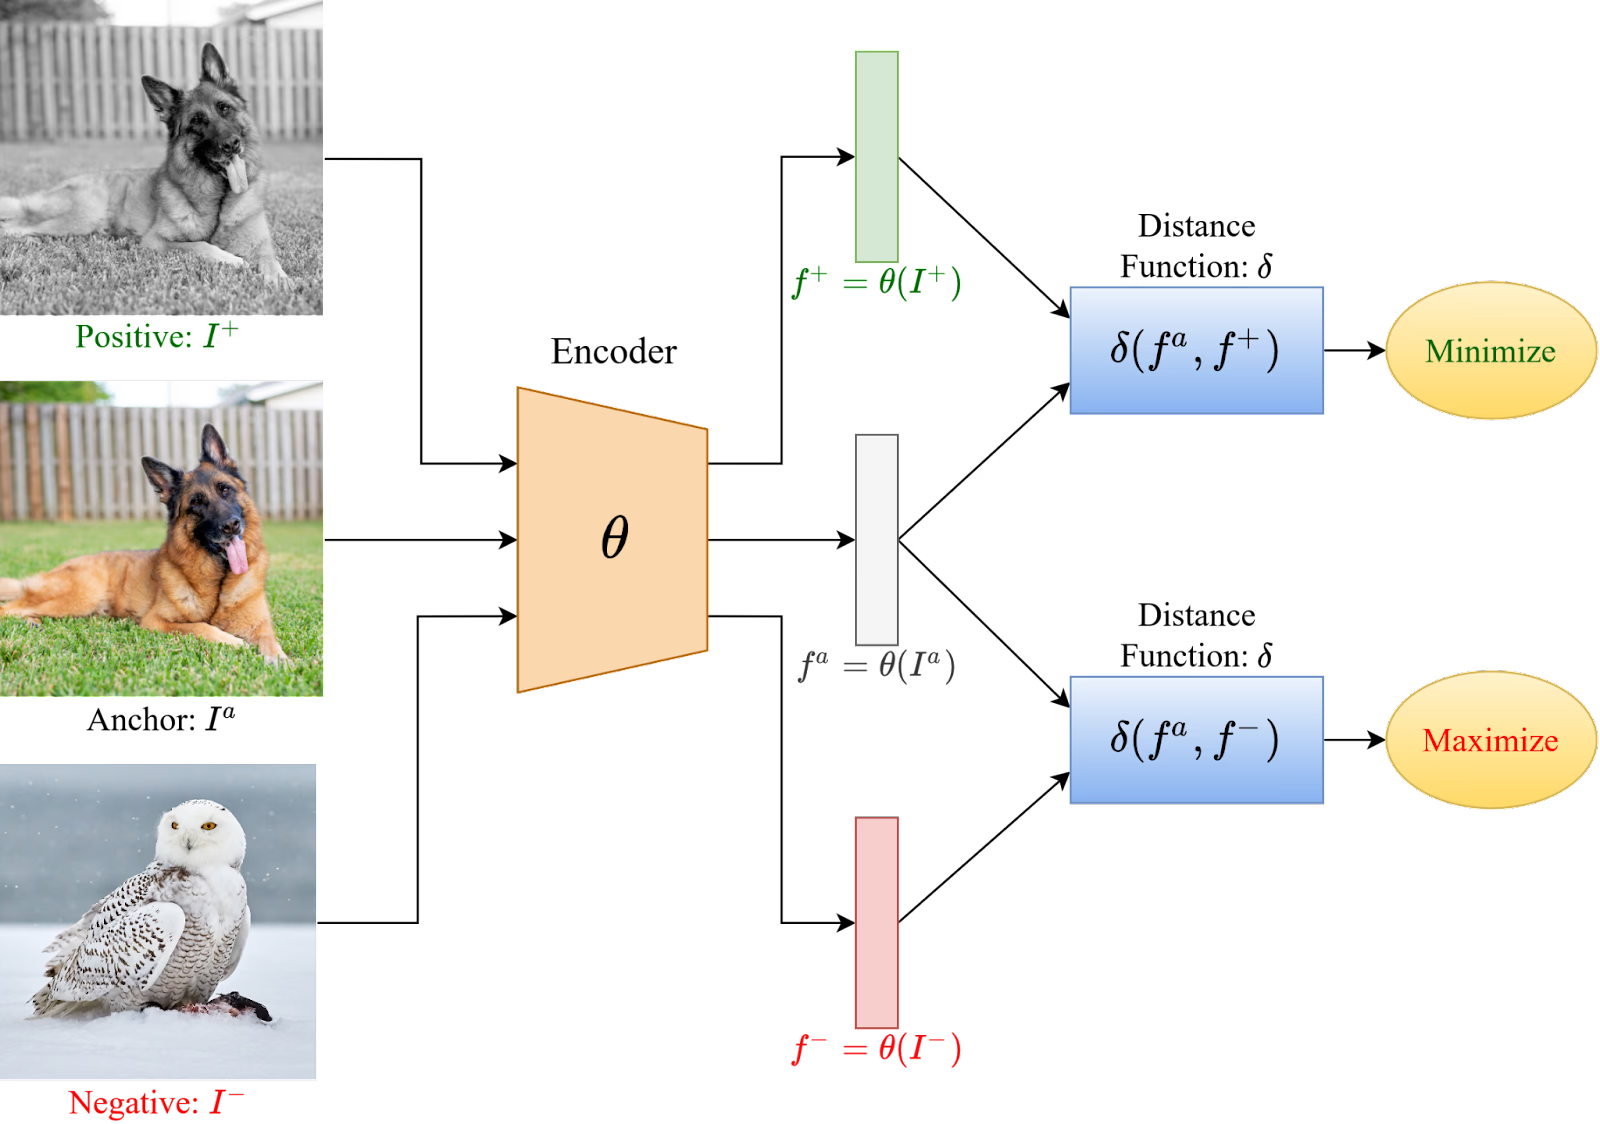
\includegraphics[width=0.8\textwidth]{img/CLearning.png}
    \caption{Conceptual representation of Contrastive Learning}
\end{figure}

\subsection{CLIP}
CLIP, which stands for Contrastive Language-Image Pre-training, is a neural network architecture developed by OpenAI\cite{CLIP} that uses Contrastive Learning to connect textual and visual information. The main idea behind CLIP is that visual and textual embeddings lives in the same feature space. Given the textual description of an image and the image itself, the embeddings returned by the model should be close together in the feature space. In few words, CLIP is trained to predict which images are most relevant to a given text prompt, and vice versa.

\begin{figure}[H]
    \centering
    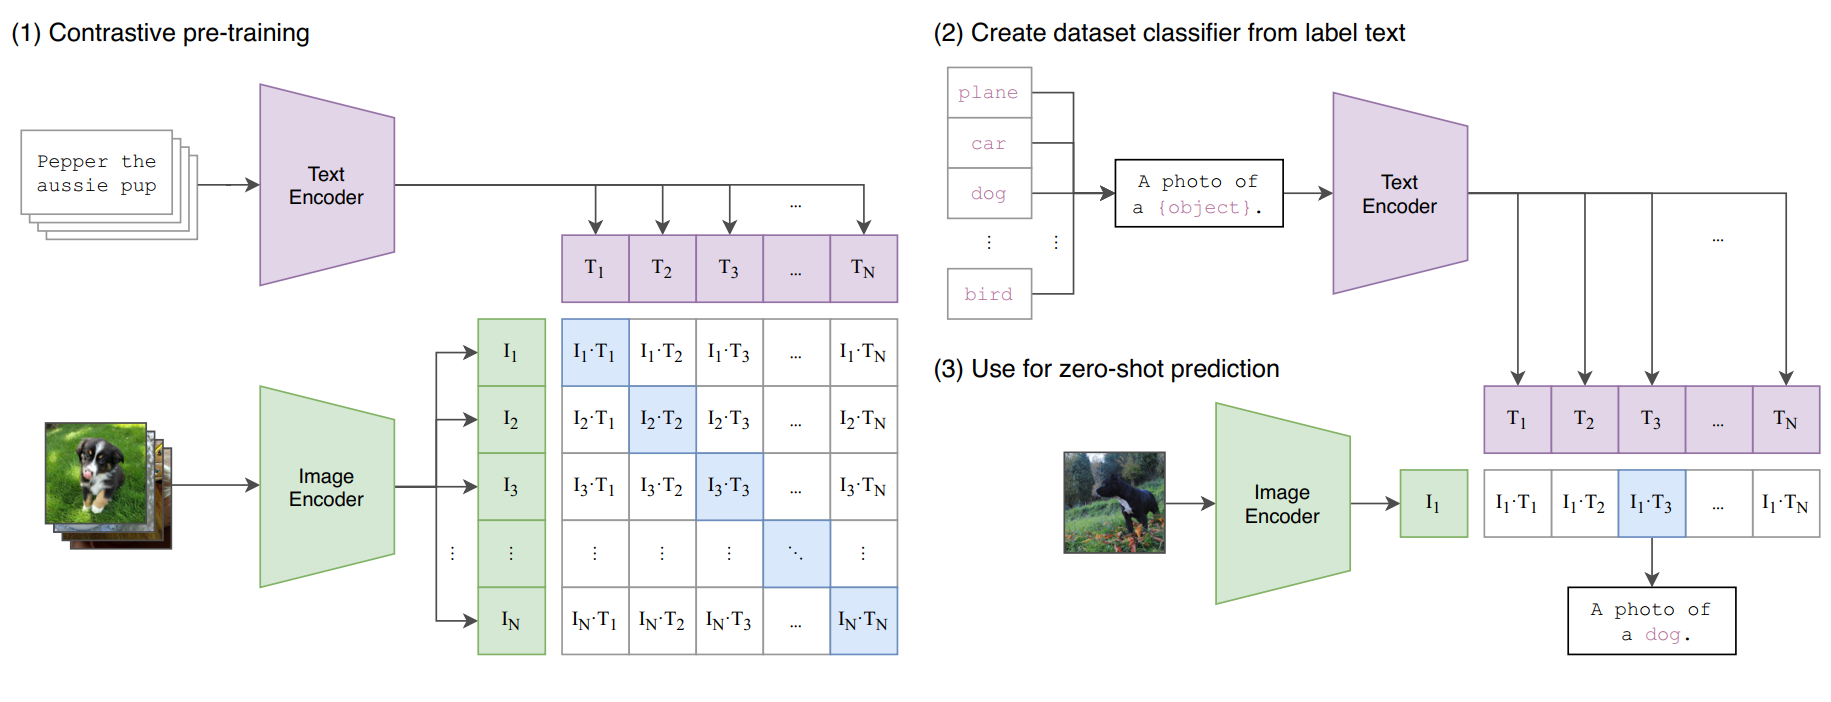
\includegraphics[width=0.8\textwidth, height=0.25\textheight]{img/CLIP.png}
    \caption{Conceptual representation of CLIP architecture}
\end{figure}

\subsection{AudioCLIP}
\label{sec:AudioClip}
AudioCLIP \cite{AudioCLIP} is an extension of the CLIP model that incorporates an additional audio modality, enabling it to understand and relate audio data alongside text and images. The architecture of AudioCLIP consists of three main components:
\begin{itemize}
    \item \textbf{A CLIP Model} to handle text and image modalities. In particual a ResNet based CLIP model is used
    \item \textbf{Audio Encoder} to handle audio modality. In particular an ESResNetXt model is used
\end{itemize}
The idea to realize AudioCLIP is very simple: in addition to the text-image contrastive loss used in CLIP, two additional loss were added: \textbf{text-audio} and \textbf{image-audio} contrastive loss. In this way the three modalities are connected in the same feature space. The training procedure of AudioCLIP consists of different main steps:
\begin{itemize}
    \item \textbf{Audio-Head Pre-Training}  
    \begin{itemize}
        \item \textbf{Standalone}: The audio head (based on ESResNeXt) is first pre-trained independently on the \textit{AudioSet} dataset.  
        \item \textbf{Cooperative}:  
        \begin{itemize}
            \item The classification layer of the pre-trained audio head is replaced with a randomly initialized layer whose output size matches CLIP’s embedding space.  
            \item The audio head is then trained jointly with the frozen text and image heads, in a \textit{multi-modal knowledge distillation} setup, making audio embeddings compatible with CLIP embeddings.
        \end{itemize}
    \end{itemize}

    \item \textbf{AudioCLIP Training}  
    \begin{itemize}
        \item After making the audio head compatible with CLIP, the entire tri-modal model (audio, text, image) is trained on \textit{AudioSet}.  
        \item All three modality-specific heads are updated together, allowing the model to adapt to the distributions of audio samples, image frames, and textual class names.  
        \item This joint training improves performance compared to training only the audio head.
    \end{itemize}
\end{itemize}


\begin{figure}[H]
    \centering
    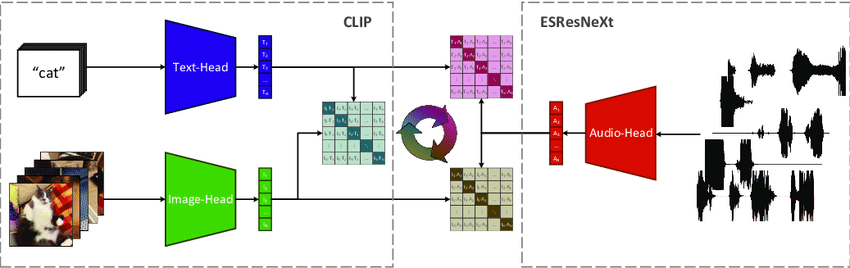
\includegraphics[width=0.8\textwidth]{img/AudioCLIP.png}
    \caption{Conceptual representation of AudioCLIP architecture}
\end{figure}
\newpage
\section{Contrastive Learning arcitetures in Multimodal Recommender Systems}
CLIP and AudioCLIP were born, and mainly used, for classification tasks. However, their ability to create a shared feature space for different modalities makes them suitable for multimodal recommender systems as well.
\subsection{CLIP in Multimodal Recommender Systems}
Zixuan Yi et al. \cite{CLIPRecSys} analyzed the use of CLIP in multimodal recommender systems. Up to few years ago, multimodal features were extracted using pretrained models on a single modality, such as ResNet for images and BERT for text. This leads to a problem: the features extracted from different modalities are not aligned in the same feature space. To solve this problem, they proposed to use CLIP to extract aligned image and text features. In particular, they used both a frozen and a fine-tuned CLIP model to extract image and text features. Experiments involved five multimodal recommender systems: VBPR, MMGCN, MMGCL , SLMRec  and LATTICE and showed that both frozen and fine-tuned CLIP features significantly outperformed the traditional pretrained features in four out of five models. To be more specific, due to it's learning objective, LATTICE perform better without CLIP features. The fine-tune algorithm proposed by the authors is known as \textbf{END-TO-END Training}.
\paragraph{End-To-End Training}
The end-to-end fine-tuning procedure integrates the CLIP encoder directly into the recommendation model and jointly optimizes both components using recommendation losses. The training steps are as follows:

\begin{enumerate}
    \item \textbf{Load Data:} Prepare the dataset by loading raw data
    
    \item \textbf{Initialize CLIP Encoder:} Load a pre-trained CLIP model and its corresponding weights.
    
    \item \textbf{Generate Embeddings:} Use the CLIP encoder to extract image embeddings and text embeddings from the dataset:
    
    \item \textbf{Integrate Embeddings:} Feed the extracted embeddings into the recommendation model as initial item representations.
    
    \item \textbf{Joint Optimisation:} For each training epoch, jointly update both the CLIP encoder and the recommendation model:
    \begin{enumerate}
        \item Perform a forward pass to compute user--item scores.
        \item Compute the recommendation loss 
        \item Backpropagate the loss and update both the CLIP encoder and recommendation model parameters:
    \end{enumerate}
    \item \textbf{Evaluation:} After each epoch, evaluate and log recommendation performance metrics (e.g., NDCG, Recall) to monitor progress.
\end{enumerate}

This end-to-end strategy allows the CLIP encoder to adapt its visual and textual representations specifically to the recommendation task, leading to improved alignment between modalities and better overall recommendation performance.
\subsection{AudioCLIP in Multimodal Recommender Systems}
In literature there are evidence of the use of AudioCLIP in multimodal recommender systems.

\bibliographystyle{plain}
\bibliography{biblio.bib}

\end{document}
